% !TEX root = ../Dokumentation.tex
\subsection{Lenkung}
\textbf{Funktionsbeschrieb}\\[0.2cm]
Die Lenkung ist eine Achsschenkellenkung. Sie wird heute in fast allen PKWs, LKWs, Omnibussen und sonstigen Nutzfahrzeugen eingesetzt. Bei dieser Art der Lenkung befinden sich die Räder auf einzeln lenkbaren Achsschenkeln, die jeweils mit einem Spurstangenhebel versehen sind. Die Spurstangenhebel sind ungefähr senkrecht zur Vorderachse bzw. ungefähr parallel zur Längsachse des Fahrzeugs ausgerichtet und durch eine Spurstange miteinander verbunden. Deshalb ist es möglich beide Räder gleichzeitig zu lenken.\\[0.2cm]
\begin{figure}[H]%Position festigen
\centering
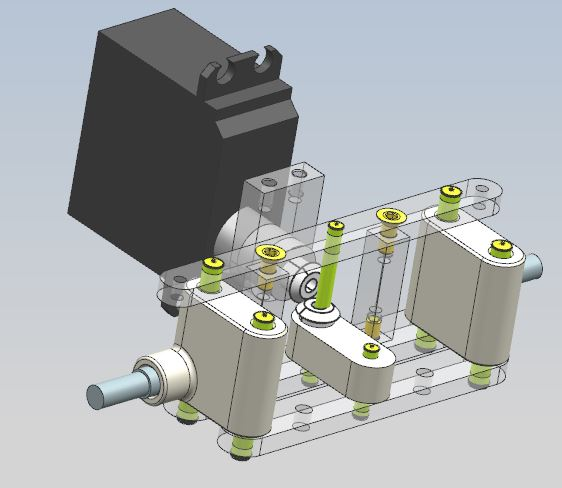
\includegraphics[width=0.7\textwidth]{03_Loesungskonzept/pictures2/Lenkung.JPG}
\caption{Achsschenkellenkung}
\label{fig:activityRoute}
\end{figure}
\begin{figure}[H]%Position festigen
\centering
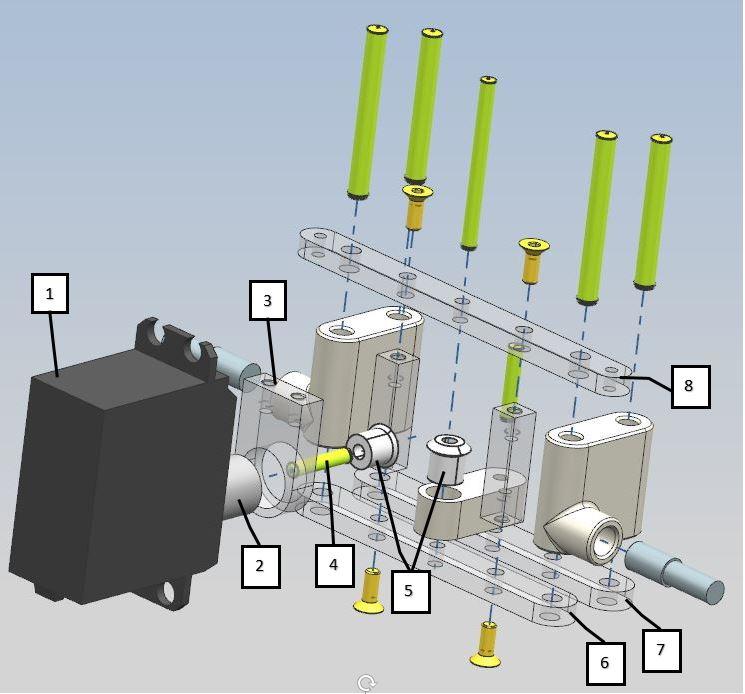
\includegraphics[width=0.7\textwidth]{03_Loesungskonzept/pictures2/Lenkung_Explosion_1_lg.JPG}
\caption{Achsschenkellenkung mit Komponentenbeschriftung 1}
\label{fig:activityRoute}
\end{figure}
\begin{figure}[H]%Position festigen
\centering
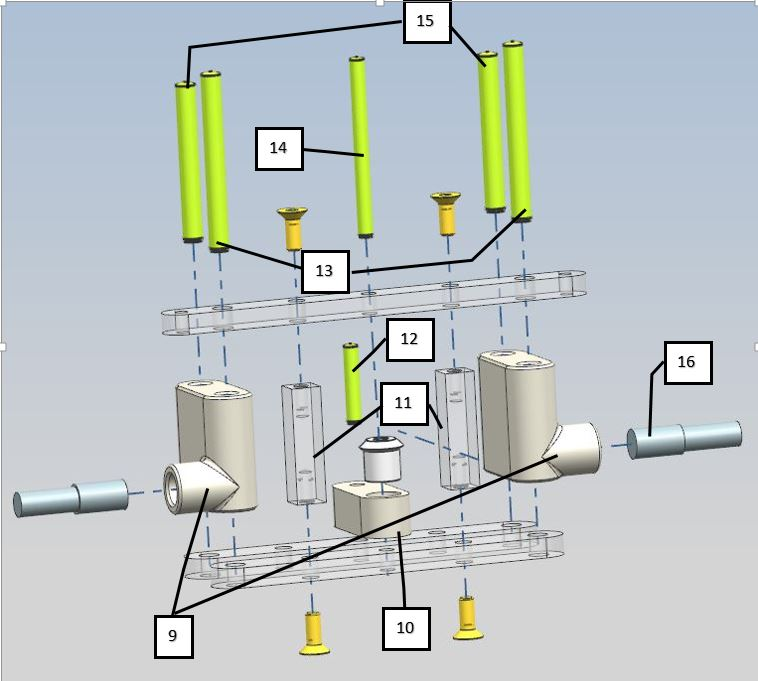
\includegraphics[width=0.7\textwidth]{03_Loesungskonzept/pictures2/Lenkung_Explosion_2_lg.JPG}
\caption{Achsschenkellenkung mit Komponentenbeschriftung 2}
\label{fig:activityRoute}
\end{figure}
Mit einem Servomotor wird über eine Kegelradverbindung der Lenkschubhebel angetrieben. Dieser treibt wiederum die Spurstange an, welche die Bewegung über die Spurstangenhebel an die Räder weitergibt.\\[0.2cm]
\textbf{Positionsnummernbeschrieb}\\[0.2cm]
Pos.1 	Servomotor Lenkung\\
Pos.2 	Verbindung Servomotor und Kegelrad\\
Pos.3 	Halterung für Kegelrad\\
Pos.4 	Achse zur Verbindung Servo mit Kegelrad\\
Pos.5 	Kegelrad m=0.5, i=1, z=16\\
Pos.6 	Starrachse 1\\
Pos.7 	Spurstange\\
Pos.8	Starrachse 2\\
Pos.9	Schubstangenhebel links und rechts\\
Pos.10	Lenkschubstange\\
Pos.11	Abstandhalter\\
Pos.12	Stift D=3mm L=16mm für Verbindung Lenkschubstange und Spurstange\\
Pos.13	Stift D=4mm L=36mm\\
Pos.14	Stift D=3mm L=36mm\\
Pos.15	Stift D=4mm L=32mm\\
Pos.16	Vorderachse\\
\newpage
\textbf{Fertigung, Beschaffung und Material}\\[0.2cm]
Pos.1 	Bezogen über HSLU\\
Pos.2 	Werkstadtfertigung HSLU / AlMgSi1 Profil D12\\
Pos.3 	Laserschneiden HSLU / Acrylglas 6mm\\
Pos.4 	Rohmaterial von HSLU selbst bearbeitet / S235JRG2C D=3mm\\
Pos.5 	Bestellt bei Mädler / Kegelräder aus Azetalharz\\
Pos.6 	Laserschneiden HSLU / Acrylglas 4mm\\
Pos.7 	Laserschneiden HSLU / Acrylglas 4mm\\
Pos.8	Laserschneiden HSLU / Acrylglas 4mm\\
Pos.9 	3D-Druck HSLU\\
Pos.10	3D-Druck HSLU\\
Pos.11	Laserschneiden HSLU / Acrylglas 6mm\\
Pos.12	Rohmaterial von HSLU selbst bearbeitet / S235JRG2C D=3mm\\
Pos.13	Rohmaterial von HSLU selbst bearbeitet / S235JRG2C D=4mm\\
Pos.14	Rohmaterial von HSLU selbst bearbeitet / S235JRG2C D=3mm\\
Pos.15	Rohmaterial von HSLU selbst bearbeitet / S235JRG2C D=4mm\\
Pos.16	Werkstadtfertigung HSLU / S235JRG2C\\
Bemerkung: Alle Fertigungszeichnungen sowie Bestelllisten für Dritthersteller, 3D-Druckteile und Laserteile sind im Anhang.\\[0.2cm]
\textbf{Schwierigkeiten}\\[0.2cm]
Bei der Lenkung gab es zwei Probleme zu überwinden. Die Spurstange (Pos.7) und die Starrachse 1 (Pos.6) welche Baugleich sind waren zu filigran. Bei schneiden der Gewinde Brach eine von ihnen. Darum wurden die Breite von 8mm auf 10mm erhöht.\\
Das jedoch weitaus schlimmere Problem, war das übertragen des Momentes über die Kegelräder. Da der Achsabstand zwischen den Kegelrädern nicht durch zu ungenaue Produktion nicht genau passten, hatten diese zu viel Spiel. Dies führte dazu, dass die Kegelräder bei höherer Belastung Zähne übersprangen. Durch unterlegen von dünnen Folien, konnte dieses Spiel so verringert werden, dass die Kegelräder das Moment übertragen können.\\[0.2cm] 
\textbf{Vergleich Konzept und Umsetzung}\\[0.2cm]
Wie unter dem Punkt Probleme schon erwähnt, wurde die Breite der Spurstange und der Starrachse 1 erhöht. Zur zusätzlichen Stabilisation der Lenkung wurden die zwei Abstandshalter (Pos.11) eingebaut.\\[0.2cm]
\textbf{Berechnungen}\\[0.2cm]
Berechnung Drehmoment Servo Lenkung
\begin{itemize}
\item Gewichtskraft auf jedes Rad $Fg = \frac{m\cdot g}{4}$
\item Abstand $l = 30mm$
\item $M = 2\cdot Fg\cdot l = 0.37Nm$
\item Sicherheitsfaktor = 1.5 (da Beschleunigung- und Bremskräfte vernachlässigt werden)
\item $M = 0.37\cdot 1.5 = 0.555Nm = 55.5Ncm$
\end{itemize}